\chapter{Testing and Results}\label{chap:testing}
In this chapter testing of the modules is explained. The complete Observer-Controller architecture is still in development stage, so the integration testing of the complete architecture described previously was not possible. So the user-level Synchronization module(Synchronization 1) is tested separately from the kernel Synchronization module (Synchronization 2). The user-level component is tested to make sure the dataspace  access is possible and it can communicate with the \texttt{Controller} via the dataspace.

To test the kernel ready queue update mechanism as a standalone component, the Genode thread ids need to be sent from a user-level component. Therefore, a new Genode component called \texttt{gehello} was developed as a utility to test the kernel module. It creates a set of threads and passes them to the kernel. In order to obtain the thread ids required Genode's trace facility is extended to get the thread ids from platform thread class of Genode OS framework which is explained in the next section.

\section{Test Utility Using Trace: gehello}

\begin{figure}[h]
\centering
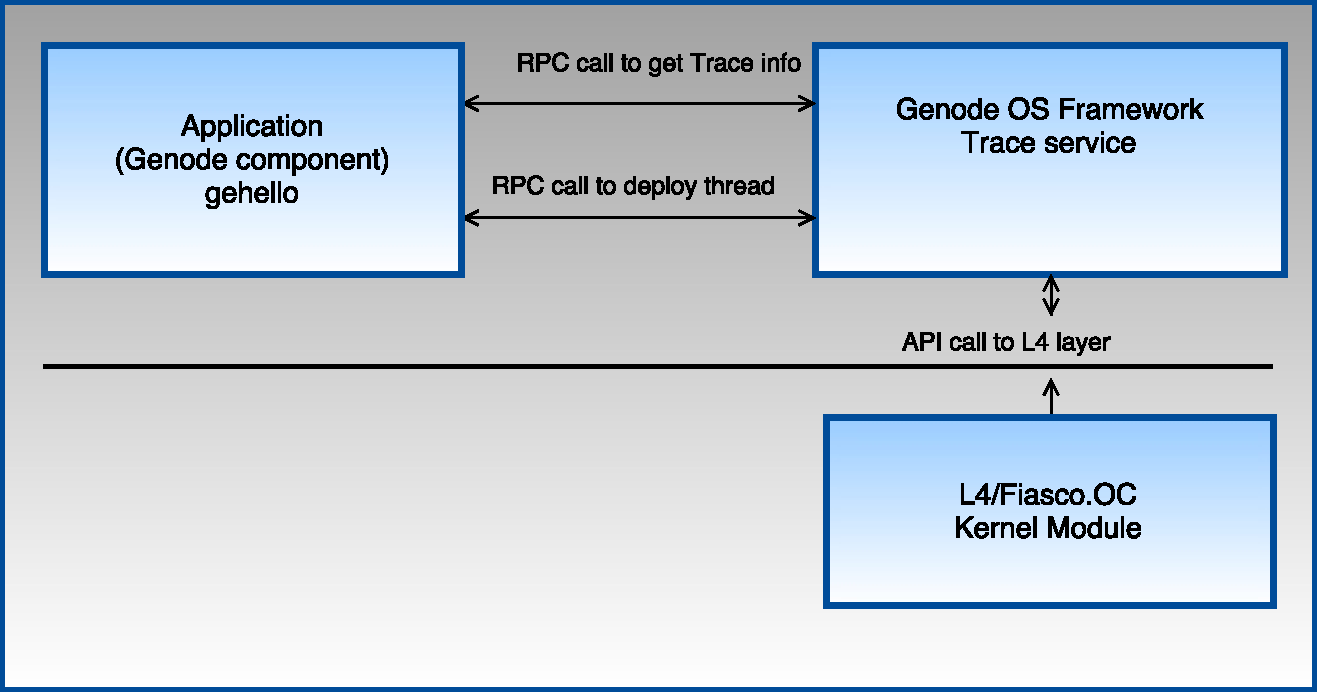
\includegraphics[width=0.7\linewidth]{figures/test1}
\caption{Test utility design using Trace service}
\label{fig:test}
\end{figure}

The gehello test utility is implemented as a Genode component, it creates a set of threads and passes them to the kernel module to update them to the ready queue. In order to create the threads, it has to inherit the Genode's thread class and specify the stack size as a template parameter. 

The Listing \ref{gehello} shows this thread creation. The class \texttt{Mythread} inherits the Genode's Thread class. It has a constructor, which in turn calls the base class's constructor with a string (name of the thread) as a parameter. This call goes to platform thread class to create the thread as explained in section \ref{foundations:thread_creation}. The entry function of this thread just does a print on the  command line. The \texttt{Thread\_creator} class creates the \texttt{Mythread} class object(myt). It has a run\_thread function which calls the start method associated with the thread. The start method invokes the entry function defined in the \texttt{Mythread} class and it has to call join method of the thread to end specify the end of thread's execution.

\begin{lstlisting}[caption={gehello trace utility},label={gehello}, style=customcpp]
class Mythread : public Genode::Thread<2*4096>
{
	public:
		Mythread() : Thread("MyThread") { }
		void entry(){
			printf("I'm a thread\n");
			// Some useful work
		}
};
class Thread_creator
{
	Mythread myt;
	public:
		int run_thread(){
				myt.start();
				Genode::Thread_capability mycap = myt.cap();
				PINF("Got Thread capability information. %lx\n", myt.tid());
				myt.join();
		}
};
\end{lstlisting}

\subsection{Trace Extension}
The information about the Genode's tasks/thread can be obtained from using Core's Trace service. Trace service was extended to get the thread information from Genode's platform thread class. 

The \texttt{source\_registry.h} has a information struct called \texttt{Info}, which is returned by Trace service to an application. A new element has been added to the Info struct for thread id. 


\begin{lstlisting}[style=customcpp]
	struct Info
		{
			Session_label      label;
			Thread_name        name;
			Execution_time     execution_time;
			Affinity::Location affinity;
			unsigned 		   prio;
			unsigned long	   thread_id;
		};
\end{lstlisting}


The \texttt{info()} method of the \texttt{subject\_registry} calls the {trace\_source\_info()} function of the \texttt{Cpu\_session\_component} class to obtain the thread information. The class \texttt{Cpu\_session\_component} has the \texttt{platform thread} object and returns the thread id.

\begin{lstlisting}[style=customcpp]
	Trace::Source::Info trace_source_info() const
			{
				return { _session_label, _name,
				         _platform_thread.execution_time(),
				         _platform_thread.affinity(),
						 _platform_thread.prio(),
						 _platform_thread.thread_id()};
			}
\end{lstlisting}


Platform thread class is extended with a method to return the thread's local id as shown below.

\begin{lstlisting}[style=customcpp]
unsigned long Platform_thread::thread_id() const
{
	return _thread.local.dst();
}
\end{lstlisting}

\section{Building the System}
The Synchronization module is tested on Ubuntu 14.04 LTS using QEMU to virtualize the hardware (PBX-A9) board. The following subsections explain the installing dependencies and compiling Genode along with the Fiasco.OC.

The changed Fiasco.OC and Genode source can be downloaded from \cite{git_synccode}.

\subsection{Installing Dependencies}

Genode and Fiasco.OC require these following packages to be installed.

\begin{itemize}

\item GNU Make version 3.81 or newer

\item libSDL-dev

\item tclsh and expect

\item byacc

\item QEMU: Required fir virtualizing the hardware.
\end{itemize}

Another option is to install the pre-compiled Genode tool chain for Linux available in Genode \href{http://genode.org/download/tool-chain}{website}.

\subsection{Compiling the gehello Application}
After installing the dependencies, clone the Genode operating system branch \texttt{focnados} from GitHub \href{https://github.com/702nADOS/genode-Synchronization}{repository}.

Once the Genode is downloaded prepare the Fiasco.OC kernel by issuing \textit{make-prepare} command in \textit{repos/base-focnados} folder.  But this would use the default Fiasco.OC code. In order to use the modified code for the thesis the \textit{port/focnados.port} file should be updated to access the code from the above mentioned GitHub repository.

Create a build directory using Genode tool for pbxa9 board using the below command
\begin{verbatim}
$ ./tool/create_builddir focnados_pbxa9
\end{verbatim}

The \texttt{gehello} application exists in the repos folder. By issuing the below make command in the build directory, the \texttt{gehello}  application can be built and tested. The expected output is given in the section \ref{testing:results}.

\begin{verbatim}
$ make -j4 run/gehello
\end{verbatim}

\section{Results}\label{testing:results}
The \texttt{gehello} application creates five threads and the Trace service returns the thread information to the user-space application. Listing \ref{gehellotrace} shows the information returned from the Trace. The names are compared to find out the threads created by the \texttt{gehello} application and these thread ids are selected and sent to the kernel using the Genode API. 

\begin{lstlisting}[caption={The returned information from the Trace service},label={gehellotrace}, style=customcpp]
ID:11 0 prio:128  thread_id: 293000 init 
ID:9 0 prio:128  thread_id: 2c0000 init -> gehello name:gehello
ID:8 0 prio:128  thread_id: 2e1000 init -> gehello name:MyThread
ID:7 0 prio:128  thread_id: 2e6000 init -> timer name:timer_drv_ep
ID:6 0 prio:128  thread_id: 2ec000 init -> gehello name:MyThread
ID:5 0 prio:128  thread_id: 2f6000 init -> gehello name:MyThread
ID:4 0 prio:128  thread_id: 2fd000 init -> timer name:timeout_scheduler
ID:3 0 prio:128  thread_id: 301000 init -> gehello name:MyThread
ID:2 0 prio:128  thread_id: 30b000 init -> gehello name:MyThread
ID:1 0 prio:128  thread_id: 317000 init -> timer name:signal handler
ID:0 0 prio:128  thread_id: 32c000 init -> gehello name:signal handler
\end{lstlisting}

The kernel threads are then identified in the kernel and added to the run queue. Listing \ref{kernelthreads} shows the kernel thread ids and the updated ready queue, when updating single thread at a time and  the updated threads start execution when the \texttt{gehello} application starts the threads.

\begin{lstlisting}[caption={The kernel thread ids and ready queue update},label={kernelthreads}, style=customcpp]

[Scheduler:sys_deploy] Thread to be scheduled: cd
fp_rq: cd => d => e9 => end

[Scheduler:sys_deploy] Thread to be scheduled: d8
fp_rq: d8 => cd => d => e9 => end

[Scheduler:sys_deploy] Thread to be scheduled: e2
fp_rq: e2 => d8 => cd => d => e9 => end

The thread execution:
[Platform_thread: start] 2e1000 started!
[init -> gehello] Got Thread capability information. c000

[init -> gehello] I am a thread!

[Platform_thread: start] 2ec000 started!
[init -> gehello] Got Thread capability information. f000

[init -> gehello] I am a thread!
\end{lstlisting}

